\documentclass{article}

\usepackage{amsmath}
\usepackage{amssymb}
\usepackage{graphicx}

\newcommand{\stencil}{
\ensuremath{\frac{1}{h^2}\begin{bmatrix}
  & 1  &   \\
1 & -4 & 1 \\
  & 1  &   
\end{bmatrix}
}}
\newcommand{\grad}{\ensuremath{\nabla}}


\begin{document}
\title{APMA4301: Problem Set 3}
\author{Brian Dawes}
\maketitle

\section*{Problem 1}
\subsection*{(a)}
\subsubsection*{i.}
\begin{align}
\nabla_5^2 u_{ij}=\frac{1}{h^2}&\big[(\sin[n\pi h(i-1)]+\sin[n\pi h(i+1)])\sin(m\pi hj) \nonumber\\
& +(\sin[m\pi h(j-1)]+\sin[m\pi h(j+1)])\sin(n\pi hi) \nonumber \\
& -4\sin(n\pi hi)\sin(m\pi hj)\big] 
\end{align}

But note that
\begin{equation}
\sin[n\pi h(i\pm 1)]=\sin(n\pi hi)\cos(n\pi h)\pm\cos(n\pi hi)\sin(n\pi h)
\end{equation}
\begin{equation}
\implies \sin[n\pi h(i-1)]+\sin[n\pi h(i+1)]=2\sin(n\pi hi)\cos(n\pi h)
\end{equation}
This relationship still holds with $n\to m$ and $i\to j$.
So now 
\begin{align}
\nabla_5^2 u_{ij}=\frac{1}{h^2}&\big[2\sin(n\pi hi)\cos(n\pi h)\sin(m\pi hj) \nonumber\\
& +2\sin(m\pi hj)\cos(m\pi h)\sin(n\pi hi) \nonumber \\
& -4\sin(n\pi hi)\sin(m\pi hj)\big] \nonumber \\
& =\frac{2}{h^2}[\cos(n\pi h)+\cos(m\pi h)-2]u_{ij}
\end{align}
\begin{equation}
\implies\boxed{\lambda_{mn}=\frac{2}{h^2}[\cos(n\pi h)+\cos(m\pi h)-2]}
\end{equation}
So the discretization of $\phi_{mn}$ is an eigenvector of $A$ with eigenvalue $\lambda_{mn}$ for $1\leq m\leq\frac{1}{h}$ and $1\leq n\leq\frac{1}{h}$ (since $m,n=0$ corresponds to the zero function and $m,n>\frac{1}{h}$ will reduce to a lower value of $m,n$ when discretized due to aliasing).

\subsubsection*{ii.}
\begin{equation}
||A^{-1}||_2=\max\left(\frac{1}{|\lambda_{mn|}}\right)=\max\left(\frac{h^2}{2|\cos(n\pi h)+\cos(m\pi h)-2|}\right)
\end{equation}

Since $m,n$ range from 1 to $\frac{1}{h}$, the cos terms range from just below 1 to -1. The maximum occurs when the denominator is closest to one which is at $m=n=1$.
\begin{equation}
||A^{-1}||_2=\left(\frac{-h^2}{2[\cos(\pi h)+\cos(\pi h)-2]}\right)
\end{equation}
\begin{align}
C=\lim_{h\to0}||A^{-1}||_2&=\lim_{h\to0}\left(\frac{-h^2}{2[\cos(\pi h)+\cos(\pi h)-2]}\right) \nonumber\\
&=\lim_{h\to0}\left(\frac{h}{\pi\sin(\pi h)+\pi\sin(\pi h)}\right) \nonumber\\
&=\lim_{h\to0}\left(\frac{1}{\pi^2\cos(\pi h)+\pi^2\cos(\pi h)}\right) \nonumber\\
&=\boxed{\frac{1}{2\pi^2}}
\end{align}

\subsection*{(b)}
\subsubsection*{i.}
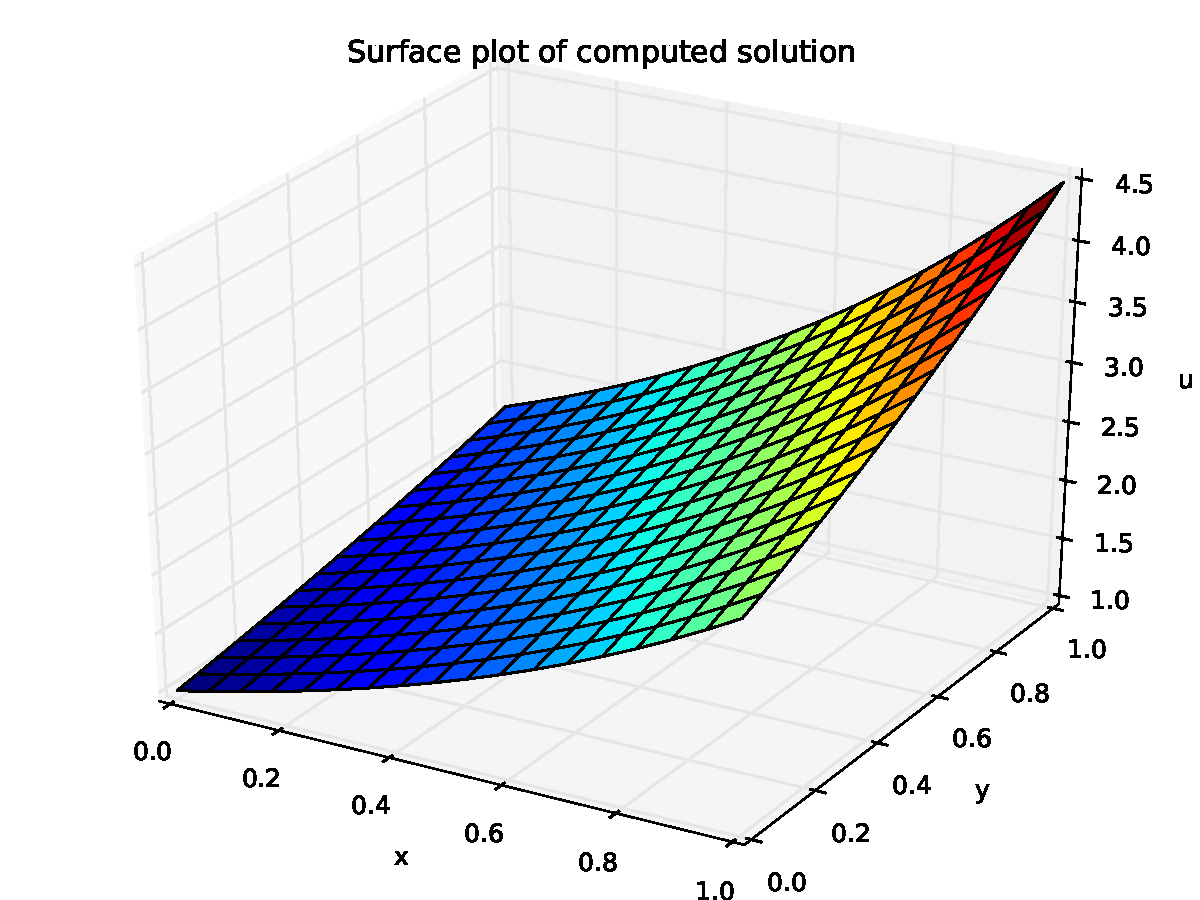
\includegraphics[width=\linewidth]{bi.pdf}
This image was generated by poisson2d\_mms.py using $h=1/16$.
\subsubsection*{ii.}
%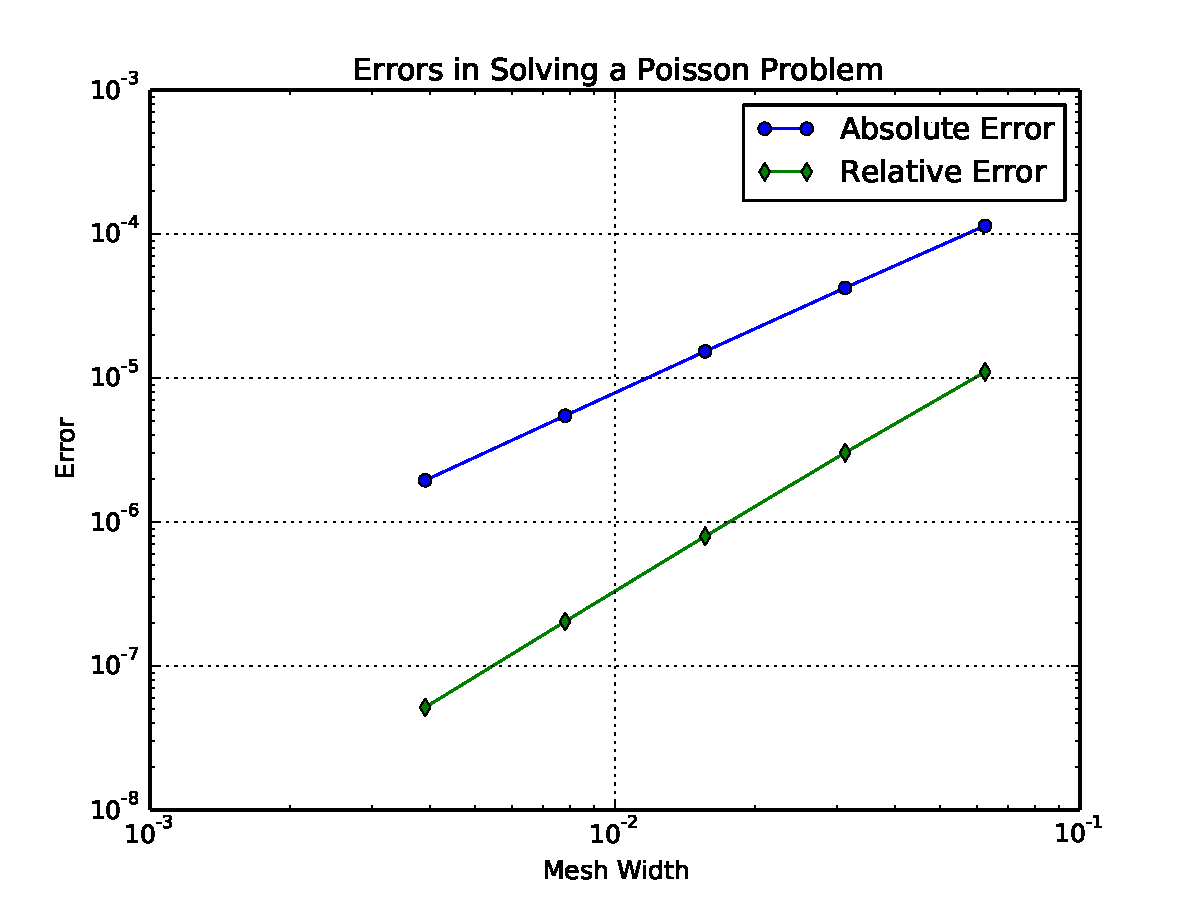
\includegraphics[width=\linewidth]{bii.pdf}
From this graph, we see the relative error is scales with , while the absolute error scales with .
\subsection*{(c)}
\subsubsection*{i.}
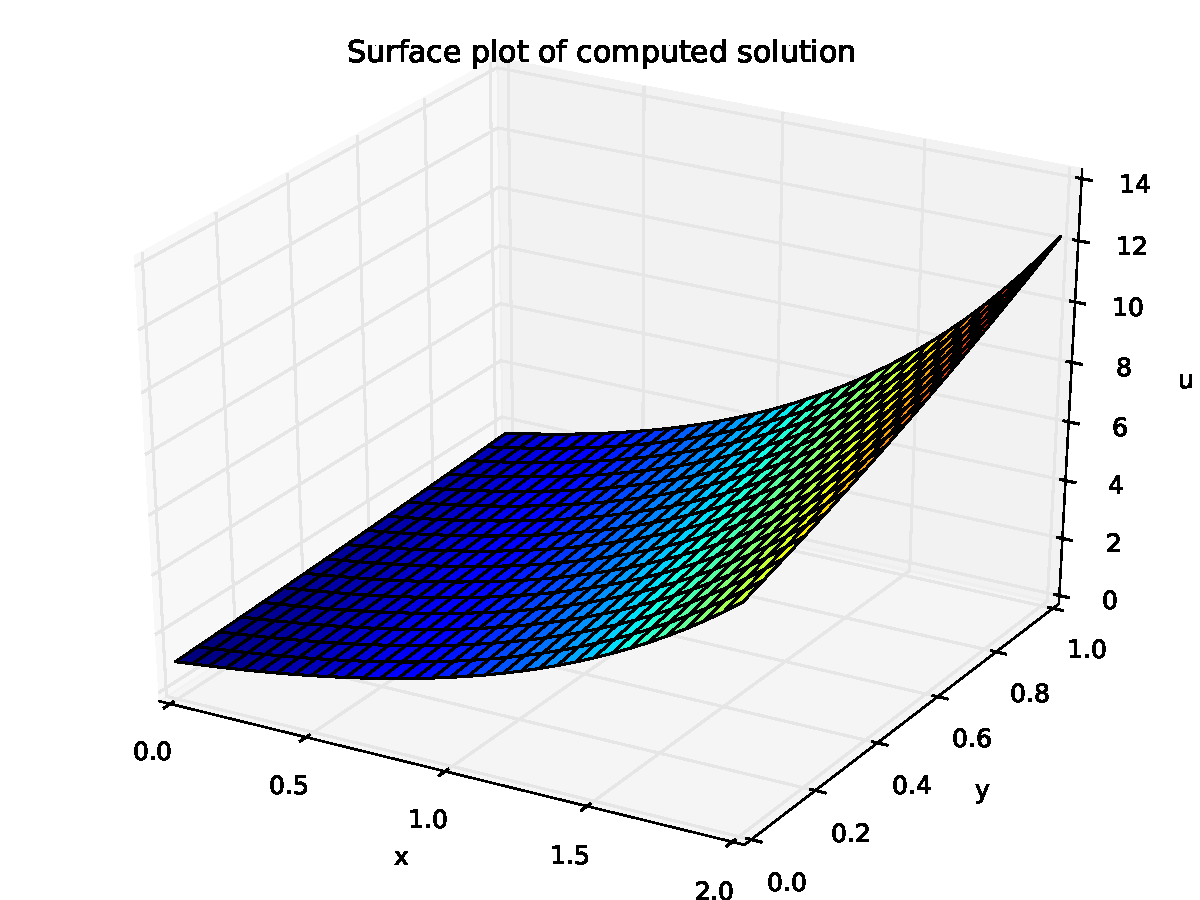
\includegraphics[width=\linewidth]{ci.pdf}
This image was generated by poisson2d\_rectangle.py using $h=1/16$
\subsubsection*{ii.}
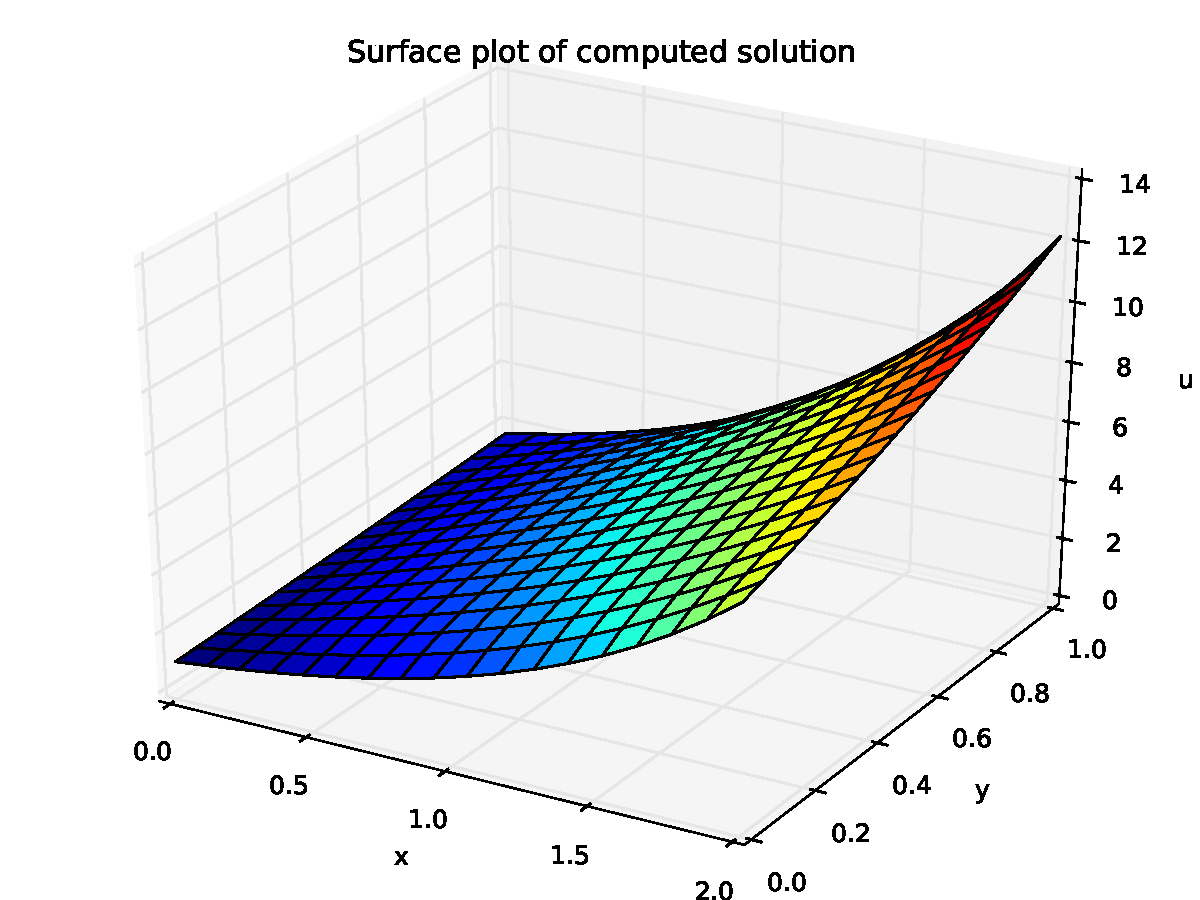
\includegraphics[width=\linewidth]{cii.pdf}
This image was generated by poisson2d\_nonuniformMesh.py using $m_x=m_y=16$
\subsubsection*{iii.}
%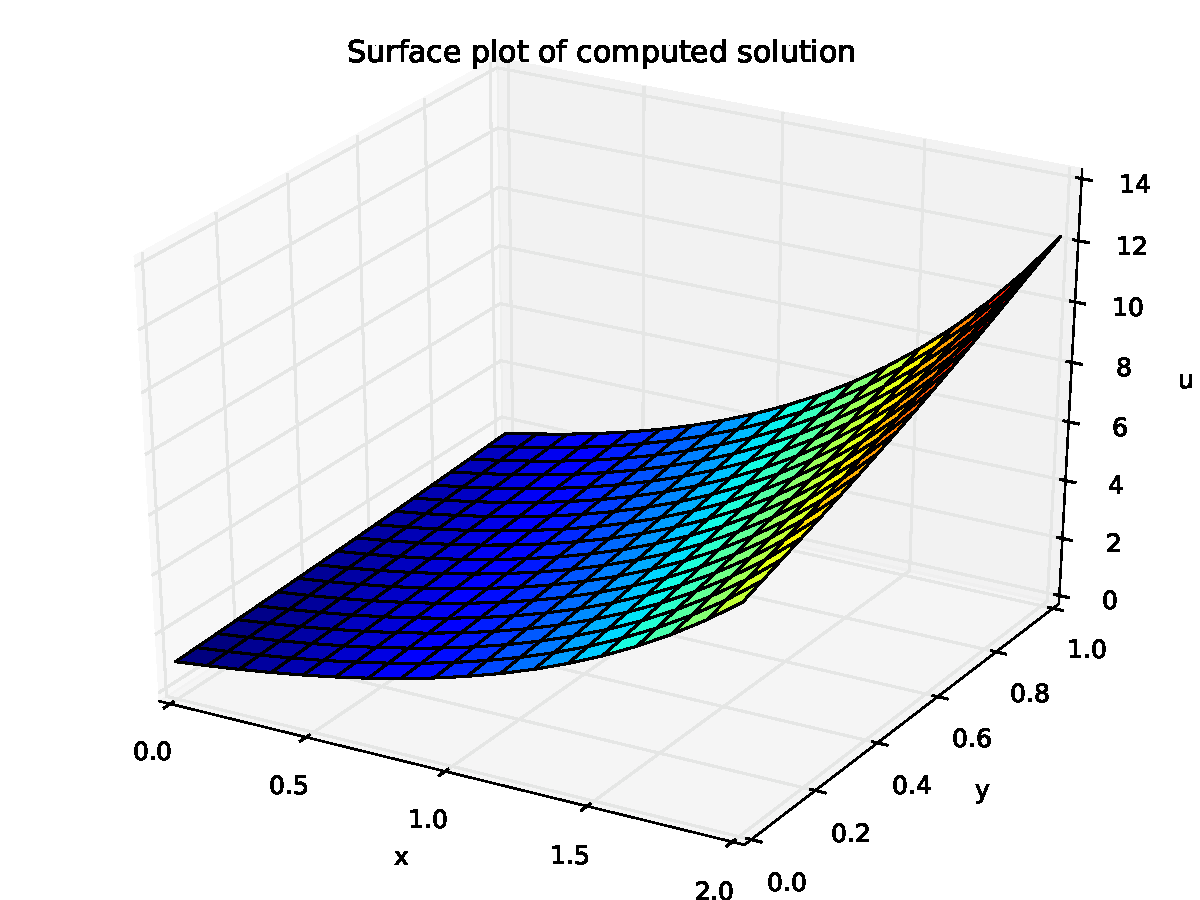
\includegraphics[width=\linewidth]{ciii.pdf}
This image was generated by poisson2d\_neumann.py using $m_x=m_y=16$
\end{document}
